\chapter{Preliminaries}

This chapter introduces all the definitions necessary to understand this document. For further details on the following concepts, refer to Reinhard Diestel’s book on graph theory~\cite{diestel2025}.
\section{Algebra Definitions}

\begin{definition}[informal]
An \emph{isomorphism} is a one-to-one correspondence (mapping) between two sets that preserves binary relationships between elements of the sets. If an element of one set is mapped to an element of the other set, this is denoted by $x \mapsto y$, meaning that the element $x$ is mapped to the element $y$.


An \emph{automorphism} is an isomorphism from a set to itself.
\end{definition}
\vspace{1em}
\begin{definition}

A \emph{group} is a set with a binary operation that satisfies the following constraints: the operation is associative, it has an identity element, and every element of the set has an inverse. For example, $(\mathbb{R}, +)$ is a group: it consists of the set of real numbers with addition as the binary operation. It has as identify element: 0, every element has an inverse element (each number with its opposite) and it's assoc iative: for all numbers $a, b, c$ in $\mathbb{R}$: $a + (b + c) = (a+b) + c$.

A \emph{homomorphism} is a transformation of one set into another that preserves in the second set the relations between elements of the first. For example, given two groups, $(G, \cdot)$ and $(H, \circ)$, a \emph{group homomorphism} from $(G, \cdot)$ to $(H, \circ)$ is a function  $\phi : G \to H$  such that $\phi(g_1 \cdot g_2) = \phi(g_1)\circ\phi(g_2)$ for every $g_1, g_2 \mathrel{\in}G_1$.

Let $(G, *)$ be a group with identity element $e$, and let $X$ be a non-empty set. A \emph{group action} of $G$ on $X$ exists if there is a map
\[
\cdot : G \times X \to X, \quad (g, x) \mapsto g \cdot x
\]
such that the following two properties hold:
\begin{enumerate}
    \item Identity: $\forall x \mathrel{\in}X, \quad e \cdot x = x$,
    \item Compatibility: $\forall g, h \mathrel{\in}G, \ \forall x \mathrel{\in}X, \quad (g * h) \cdot x = g \cdot (h \cdot x)$.
\end{enumerate}

As an example, let \emph{$S_n$} denote the \emph{symmetric group} acting on a set $X$. We indicate the action of elements of $S_n$ by exponentiation: for $x \mathrel{\in}X$ and $g \mathrel{\in}S_n$, $x^g$ denotes the image of $x$ under $g$. The same notation is used to indicate the induced action on complex structures derived from $X$. As additional notation, for $W \subseteq V$, we write $W^g = \{w^g : w \mathrel{\in}W\}$.

\end{definition}

\vspace{1em}

\begin{definition}\label{def:pointwise stabilizer}
  Let a group $G$ act on a set $X$, and let $S \subseteq X$.  
  The \emph{pointwise stabilizer} of $S$ in $G$ is the subgroup defined by:
  \[
  G_{(S)} = \{ g \in G \mid \forall x \in S,\; g \cdot x = x \}.
  \]
\end{definition}

\vspace{1em}


\begin{definition}\label{def:orbit}
    Let $G \leq S_n$ be a permutation group and let $\alpha \in \{1,\dots,n\}$. 
    The \emph{orbit} of $\alpha$ under the action of $G$ is the set
    \[
    \operatorname{Orb}_G(\alpha)=\{\alpha^g \mid g\in G\}.
    \]
    \end{definition}

    \vspace{1em}
    
    \begin{definition}\label{def:stabilizer}
    Let $G \leq S_n$ be a permutation group and let $\alpha \in \{1,\dots,n\}$. 
    The \emph{stabilizer} of $\alpha$ in $G$ is the subgroup
    \[
    G_\alpha=\{g\in G \mid \alpha^g=\alpha\}.
    \]
    \end{definition}

\section{Graph Definitions}

\begin{definition}\label{def:graph}
A \emph{graph} is a pair $G = (V, E)$ of sets satisfying $E \subseteq \binom {V}{2}$; thus, the elements of $E$ are 2-element subsets of $V$. The elements of $V$ are the \emph{vertices} of the graph $G$, the elements of $E$ are its \emph{edges}.

Let \emph{$V^*$} denote the set of finite sequences of vertices. For $\sigma \mathrel{\in}V^*$, $|\sigma|$ denotes the number of components of $\sigma$.If  $\sigma= (v_1, v_2, \ldots,v_k)  \mathrel{\in}V^*$ and $w  \mathrel{\in}V$ then  $\sigma\mid\mid w$  denotes $(v_1, v_2, \ldots ,v_k, w)$. Furthermore, for $0 \leq s \leq k$, \\
${[\sigma]}_s  \coloneqq(v_1, v_2, \ldots,v_s)$. 


An acyclic graph (one not containing any cycles) is called a \emph{forest}. 
A connected forest is called a \emph{tree}. Each vertex of a tree is called 
a \emph{node}, and a node of degree 1 (only connected to one node) is called 
a \emph{leaf}. When a particular node is designated as the starting point, 
that node is called the \emph{root}. Given a tree $T$, a \emph{subtree} $T'$ 
is a connected subgraph of $T$ that is itself a tree. We write $T' \subseteq T$ 
to denote that $T'$ is a subtree of $T$.

Let $G= (V,E)$ be a graph. Let $\sim$ be an equivalence relation on $V$. The \emph{quotient graph} of $G$ with respect to $\sim$, denoted $G/\sim$,  is a graph $ (V', E')$ such that: 
\begin{enumerate}
    \item $V' = V/{\sim} = \{[v] \mathrel{|} v \mathrel{\in} V\}$
    \item $E' = \{[u][v] \mathrel{|} uv \mathrel{\in} E\}$
\end{enumerate}
\end{definition}

\vspace{1em}

\begin{definition}\label{def:class of graphs}
We let \emph{$\mathcal{G}_n$} be the set of all graphs on $n$ vertices (without loss of generality, say $V = \{1, 2, \ldots, n\}$).\emph{$\mathcal{G}$} represents the set of all graphs.
\end{definition}

\vspace{1em}

\begin{definition}\label{def:$K1_3$}

The \emph{star graph} $K_{1,3}$ is a tree with one internal node and three leaves. It is also known as the \emph{claw graph}. The internal node is called the \emph{center} of the star graph. Pour la majorité de nos exemples, nous allons utiliser ce graphe.

\begin{figure}[ht]
    \centering
        \begin{tikzpicture}
    \node[circle, draw] (v0) at (0,0) {};
    \node[circle, draw] (v1) at (0,1.5) {};
    \node[circle, draw] (v2) at (-1.5,-1) {};
    \node[circle, draw] (v3) at (1.5,-1) {};

    \draw (v0) -- (v1);
    \draw (v0) -- (v2);
    \draw (v0) -- (v3);
\end{tikzpicture}
    \caption{The star graph $K_{1,3}$ with its center and leaves.}
\end{figure}
\end{definition}
\subsection{Definitions specifics to isomorphisms}

\vspace{1em}

\begin{definition}\label{def: colouring}
A \emph{colouring} of $V$ (or of $G \mathrel{\in}\mathcal{G}$) is a surjective function $\pi$ from $V$ onto $\{1, 2,\ldots, k\}$ for some $k$. The number of colours, i.e. $k$, is denoted by $|\pi|$. A cell of $\pi$ is the set of vertices with some given colour; that is, $\pi^{-1} (j)$ for some $j$ with $1 \mathrel{\leq} j \mathrel{\leq} |\pi|$. We let $\Pi$ be the set of all colourings.

If $\pi$, $\pi'$ are colourings, then $\pi'$ is \emph{finer than or equal} to $\pi$, written $\pi' \preccurlyeq\pi$, if $\pi(v) < \pi(w) \Rightarrow\pi' (v) < \pi' (w)$ for all $v, w \mathrel{\in}V$ (This implies that each cell of $\pi'$ is a subset of a cell of $\pi$).

Here, the colouring is not related to a \textit{proper colouring}, $\pi$ is related to a \textit{partitioning}. 

A \emph{discrete colouring} is a colouring in which each cell is a singleton, in which case $|\pi|= n$.

A \emph{coloured graph} is a pair $ (G, \pi)$ where $\pi$ is a colouring of $G$.

A colouring of a graph is called \emph{equitable} if any two vertices of the same colour are adjacent to the same number of vertices of each colour. This is also called an \emph{equitable/stable partition}.
\end{definition}

\vspace{1em}

\begin{definition}\label{def: action group/automorphism group}
Let \emph{$S_n$} denote the \emph{symmetric group} acting on $V$.

There are several notations to consider:
    \begin{enumerate}
        \item if $\pi$ is a colouring of $V$, then $\pi^g$ is the colouring with $\pi^g (v^g) =
        \pi(v)$ for each $v \mathrel{\in}V$.
        \item if $ (G,\pi)$ is a coloured graph, then $ {(G,\pi)}^g = (G^g,\pi^g)$.
    \end{enumerate}

These properties show that two coloured graphs $ (G, \pi)$ and $ (G', \pi')$ are isomorphic iff there exists $g \mathrel{\in}S_n$ such that $ (G', \pi') = {(G, \pi)}^g$. In this case, we write $ (G, \pi) \cong(G', \pi')$.


$\Aut(G,\pi) = \left\{g \mathrel{\in} S_n: {(G,\pi)}^g = (G,\pi) \right\}$; $\Aut(G,\pi)$ is the \emph{Automorphism group} of coloured graph $ (G,\pi)$.   

\end{definition}

\vspace{1em}

\begin{definition}\label{def:canonical form}

The \emph{canonical form} is a function
\[
C : \mathcal{G} \times \Pi \to \mathcal{G} \times \Pi
\]


such that for all  $G \mathrel{\in}\mathcal{G},  \pi\mathrel{\in}\Pi$ and  $g \mathrel{\in}S_n$:

\begin{enumerate}
    \item $C (G,\pi) \cong(G,\pi)$. 
    \item $C (G^g,\pi^g) = C (G,\pi)$.
\end{enumerate}
\end{definition}

\section{Complexity Definitions}

For more informations on the complexity definitions, you can refer to  Michael Sipser's book: Introduction to the Theory of Computation~\cite{sipser1996introduction}

\vspace{1em}

\begin{definition}[minimalist]\label{def:NP}
The class \emph{\NP} (comes from nondeterministic polynomial) is the set of decision problems for which the problem instances have certificates verifiable in polynomial time by a deterministic Turing machine, or alternatively the set of problems that can be solved in polynomial time by a nondeterministic Turing machine.

A decision problem  is a member of \coNP{} iff its complement is in the complexity class \NP.

A decision problem $B$ is \emph{\NP-complete} if it satisfies the two following conditions:
\begin{enumerate}
    \item $B$ must belong to the class \NP{}.
    \item Every problem in \NP{} can be reduced to $B$ in polynomial time.
\end{enumerate}
\end{definition}

\vspace{1em}

\begin{definition}
A problem is \emph{\NP-intermediate} (\NPI) if it is not \NP{}-complete nor \P. 
\end{definition}

\vspace{1em}

\begin{definition}\label{def:SPP}
    A language $L$ belongs to the class \emph{SPP} (\textbf{S}toic \textbf{PP}) if there exists a polynomial-time nondeterministic Turing machine $M$ such that
    \[
    x\in L \iff \#\mathrm{acc}_M(x)=1  \text{ and }  x\notin L \iff \#\mathrm{acc}_M(x)=0,
    \]
    where $\#\mathrm{acc}_M(x)$ denotes the number of accepting computation paths
    of $M$ on input $x$.
    \end{definition}


\vspace{1em}

\begin{definition}\label{def: logspace}
$\LOGSPACE$ (or \L) is the complexity class of decision problems that can be solved by a deterministic Turing machine using a logarithmic amount of writable memory.
\end{definition}


\vspace{1em}

\begin{definition}
An \emph{oracle} for a language $B$ is an external device that is capable of reporting whether any string $w$ is a member of $B$. An oracle Turing machine is a modified Turing machine that has the additional capability of querying an oracle. We write $M^B$ to describe an oracle Turing machine that has an oracle for language $B$.

The \emph{Polynomial-Time Hierarchy} (\PH) is a hierarchy of complexity classes that generalizes the classes \NP{} and \coNP. Formally, the base level of the hierarchy is defined as:
\[
\Delta_0^{\P} \coloneqq \Sigma_0^{\P} \coloneqq \Pi_0^{\P} \coloneqq \P,
\]

where $\P$ denotes the class of decision problems solvable in polynomial time by a deterministic Turing machine. Then, for every $i \geq 0$, the hierarchy is defined recursively as follows:

\begin{itemize}
    \item $\Delta_{i+1}^{\P} \coloneqq \P^{\Sigma_i^{\P}}$
    \item $\Sigma_{i+1}^{\P} \coloneqq \NP^{\Sigma_i^{\P}}$
    \item $\Pi_{i+1}^{\P} \coloneqq \coNP^{\Sigma_i^{\P}}$
\end{itemize}

Here, $\P^A$ denotes the class of problems solvable in polynomial time by a deterministic Turing machine equipped with an oracle for some complete problem in class $A$. The classes $\NP^A$ and $\coNP^A$ are defined analogously, using nondeterministic and co-nondeterministic Turing machines, respectively.

For example, $\Sigma_{i}^{\P} = \NP$, $\Pi_{i}^{\P} = \coNP$,  and $\Delta_{2}^{\P} \coloneqq \P^{\NP}$ is the class of problems solvable in polynomial time with access to an oracle for an \NP-complete problem.

This definition implies that each level of the hierarchy is contained within the next. That is:

\begin{itemize}
    \item $\Sigma_i^{\P} \subseteq \Delta_{i+1}^{\P} \subseteq \Sigma_{i+1}^{\P}$
    \item $\Pi_i^{\P} \subseteq \Delta_{i+1}^{\P} \subseteq \Pi_{i+1}^{\P}$
\end{itemize}

The union of all classes in this hierarchy forms the polynomial-time hierarchy, denoted by \PH{}.
\end{definition}


\vspace{1em}


\begin{figure}[H]
    \centering
    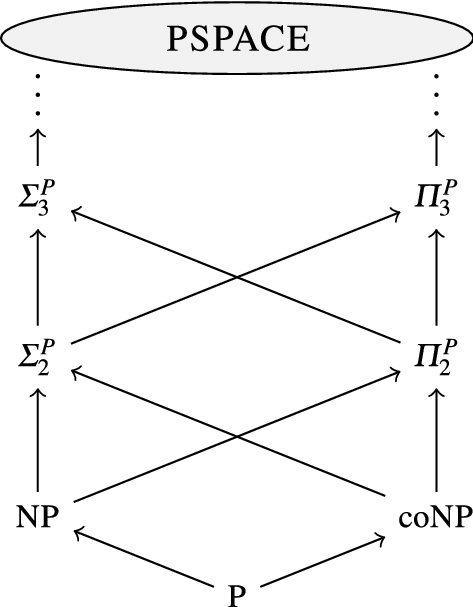
\includegraphics[width=0.6\linewidth]{imgs/Complexity-classes-the-polynomial-hierarchy-Stockmeyer-1976.png}
    \caption{Polynomial Time Hierarchy where the arrows denote the inclusion: image from~\cite{ph}}\label{fig: ph}
\end{figure}

